\documentclass[a4paper, 11pt]{article}

\usepackage{graphicx}
\usepackage{graphics}
\usepackage{verbatim}
\usepackage{listings}
\usepackage{color}
\usepackage[bitheight=6ex]{bytefield}
\usepackage[bookmarksopen=true]{hyperref}

\begin{document}

\title{SCAB: serial to CAN bridge}
\author{IGREBOT team}
\date{}

\maketitle


\newpage
\tableofcontents
\addtocontents{toc}{\protect\setcounter{tocdepth}{1}}


\newpage
\begin{abstract}
This document describes the SCAB api library and the DSPIC33F firmware.
\end{abstract}


\newpage
\section{Introduction}

\subsection{Overview}
\begin{figure}[]
\centering
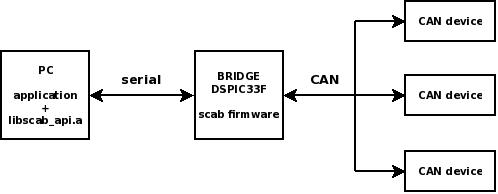
\includegraphics[scale=0.5]{./dia/scab_network/main.jpeg}
\caption{serial to CAN bridging}
\label{scab_bridging}
\end{figure}

\paragraph{}
Usually, PCs do not have the hardware interfaces required to communicate on a
CAN network. SCAB is an opensource project to add CAN connectivity to PCs by
bridging a serial port. To do so, SCAB provides the following:
\begin{itemize}
\item a firmware to be flashed on a DSPIC33F board,
\item a programming interface implemented in a library used by host applications.
\end{itemize}

\subsection{Availability}
\paragraph{}
The project is maintained in a GIT repository:
\begin{center}
\url{https://github.com/texane/scab}
\end{center}
\paragraph{}
In the remaining of this document, the expression:
\begin{center}
\$SCAB\_REPO\_DIR
\end{center}
denotes the directory where the repository was cloned.

\subsection{Dependencies}
\paragraph{}
The project depends on the following softwares:
\begin{itemize}
\item a working LINUX system with standard GNU tools,
\item MPLABX version 1.0 .
\end{itemize}
Note that WINDOWS and MACOSX are not yet supported.


\newpage
\section{Host application programming interface}

\subsection{Overview}
\paragraph{}
The source code is located in:
\begin{center}
\$SCAB\_REPO\_DIR/src/api
\end{center}

\paragraph{}
The API is shipped as a standalone static library and can be built using:\\
\begin{small}
\lstset{commentstyle=\color{blue}}
\lstset{language=C}
\begin{lstlisting}[frame=tb]
cd $SCAB_REPO_DIR/build/api ;
make ;
\end{lstlisting}
\end{small}

\paragraph{}
It produces the file:
\begin{center}
\$SCAB\_REPO\_DIR/build/api/libscab\_api.a
\end{center}

If a GNU toolchain is used, the library is linked in a client application
by adding the following flags to command line:\\
\begin{small}
\lstset{commentstyle=\color{blue}}
\lstset{language=C}
\begin{lstlisting}[frame=tb]
-L$SCAB_REPO_DIR/build/api -lscab_api
\end{lstlisting}
\end{small}

\subsection{Interface documentation}
\paragraph{}
\begin{small}
\lstset{commentstyle=\color{blue}}
\lstset{language=C}
\begin{lstlisting}[frame=tb]
int scab_open(scab_handle_t**, const char*);
int scab_close(scab_handle_t*);
int scab_sync_serial(scab_handle_t*);
int scab_read_frame(scab_handle_t*, uint16_t*, uint8_t*);
int scab_write_frame(scab_handle_t*, uint16_t, const uint8_t*);
int scab_enable_bridge(scab_handle_t*);
int scab_disable_bridge(scab_handle_t*);
int scab_set_can_filter(scab_handle_t*, uint16_t, uint16_t);
int scab_clear_can_filter(scab_handle_t*);
int scab_get_handle_fd(scab_handle_t*);
\end{lstlisting}
\end{small}

\subsection{Example program}
\paragraph{}
TODO

\subsection{Limitations}
\paragraph{}
TODO

\newpage
\section{Device firmware}

\subsection{Overview}
\paragraph{}
The firmware is a piece of software put on a DSPIC33F board to perform the forwarding
of frame to and from the host PC an the CAN network.

\paragraph{}
The source code is located in:
\begin{center}
\$SCAB\_REPO\_DIR/src/device
\end{center}

\paragraph{}
Assuming that MPLABX version 1.0 has been installed with the default paths, the firmware
can be compiled using:\\
\begin{small}
\lstset{commentstyle=\color{blue}}
\lstset{language=C}
\begin{lstlisting}[frame=tb]
cd \$SCAB_REPO_DIR/build/device.X ;
make ;
\end{lstlisting}
\end{small}

\paragraph{}
It produces the file:
\begin{center}
\$SCAB\_REPO\_DIR/build/device.X/dist/default/production/device.X.production.hex
\end{center}
which is used to program the DSPIC33F flash.

\subsection{Limitations}
\paragraph{}
TODO

\newpage
\section{Protocol between host and device}

\subsection{Overview}
\paragraph{}
All the symbolic constants used in this section can be found in the file:
\begin{center}
\$SCAB\_REPO\_DIR/src/common/scab\_common.h
\end{center}

\paragraph{}
All the packets share the same basic format and are of the same fixed length
SCAB\_CMD\_SIZE (currently 11 bytes). Thus, even for packets with smaller
payloads, SCAB\_CMD\_SIZE must be sent over the serial link.

\paragraph{}
The packets can be sorted in 2 groups:
\begin{itemize}
\item bridge management commands: set parameters such as link speeds, CAN filters ...
\item frame forwarding: actual data frame forwarding.
\end{itemize}

\paragraph{}
A management command is always sent by the host to the bridge device. It always
requires a SCAB\_CMD\_STATUS to be sent, containing the completion status of the
command.

\paragraph{}
SCAB\_CMD\_FRAME is the only non management packet. It can be sent either by the
host to send a frame on the CAN network, or by the device to forward a frame from
the CAN network to the host. There is no SCAB\_CMD\_STATUS packet involved in those
transfers.

\paragraph{}
Note that the little endian byte ordering is used between the host and the bridge.

\subsection{Packet formats}

\newpage
\subsubsection{Basic packet format}
\begin{figure}[htbp]
  \centering
  \begin{bytefield}{32}
    \bitheader{0,7-8,15-16,23-24,31} \\
    \begin{rightwordgroup}{command identifier (1 byte)}
      \bitbox{8}{\parbox{\width}{\centering \tiny{SCAB\_CMD\_xxx}}}
    \end{rightwordgroup} \\

    \begin{rightwordgroup}{command specific (10 bytes)}
      \bitbox{32}{} \\
      \bitbox{32}{} \\
      \bitbox{24}{}
    \end{rightwordgroup}
  \end{bytefield}
  \caption{Basic packet format}
  \label{fig:basic-packet-format}
\end{figure}

\paragraph{}
All the packets follow the same basic format. This format is then specialized
using the command identifier. The data field is then used according to the
command as described in the next sections.

\newpage
\subsubsection{SCAB\_CMD\_FRAME format}
\begin{figure}[htbp]
  \centering
  \begin{bytefield}{32}
    \bitheader{0,7-8,15-16,23-24,31} \\
    \bitbox{8}{\parbox{\width}{\centering \tiny{SCAB\_CMD\_FRAME}}} \\
    \bitbox{16}{\parbox{\width}{\centering \tiny{CAN SID \\ (2 bytes)}}} \\
    \begin{rightwordgroup}{CAN payload (8 bytes)}
      \bitbox{32}{} \\
      \bitbox{32}{}
    \end{rightwordgroup}
  \end{bytefield}
  \caption{SCAB\_CMD\_FRAME format}
  \label{fig:scab-cmd-frame-format}
\end{figure}

\newpage
\subsubsection{SCAB\_CMD\_SYNC format}
\begin{figure}[htbp]
  \centering
  \begin{bytefield}{32}
    \bitheader{0,7-8,15-16,23-24,31} \\
    \bitbox{8}{\parbox{\width}{\centering \tiny{SCAB\_CMD\_SYNC}}} \\
    \begin{rightwordgroup}{unused (10 bytes)}
      \bitbox{32}{} \\
      \bitbox{32}{} \\
      \bitbox{24}{}
    \end{rightwordgroup}
  \end{bytefield}
  \caption{SCAB\_CMD\_SYNC format}
  \label{fig:scab-cmd-sync-format}
\end{figure}

\newpage
\subsubsection{SCAB\_CMD\_ENABLE format}
\begin{figure}[htbp]
  \centering
  \begin{bytefield}{32}
    \bitheader{0,7-8,15-16,23-24,31} \\
    \bitbox{8}{\parbox{\width}{\centering \tiny{SCAB\_CMD\_ENABLE}}} \\
    \bitbox{8}{\parbox{\width}{\centering \tiny{boolean value \\ (1 byte)}}} \\
    \begin{rightwordgroup}{unused (9 bytes)}
      \bitbox{32}{} \\
      \bitbox{32}{} \\
      \bitbox{8}{}
    \end{rightwordgroup}
  \end{bytefield}
  \caption{SCAB\_CMD\_ENABLE format}
  \label{fig:scab-cmd-enable-format}
\end{figure}

\newpage
\subsubsection{SCAB\_CMD\_SET\_CAN\_TIMES format}
\paragraph{}
TODO, not yet implemented

\newpage
\subsubsection{SCAB\_CMD\_SET\_CAN\_FILTER format}
\begin{figure}[htbp]
  \centering
  \begin{bytefield}{32}
    \bitheader{0,7-8,15-16,23-24,31} \\
    \bitbox{8}{\parbox{\width}{\centering \tiny{SCAB\_CMD\_SET\_CAN\_FILTER}}} \\
    \bitbox{16}{\parbox{\width}{\centering \tiny{mask \\ (2 bytes)}}} \\
    \bitbox{16}{\parbox{\width}{\centering \tiny{SID \\ (2 bytes)}}} \\
    \begin{rightwordgroup}{unused (6 bytes)}
      \bitbox{32}{} \\
      \bitbox{24}{}
    \end{rightwordgroup}
  \end{bytefield}
  \caption{SCAB\_CMD\_SET\_CAN\_FILTER format}
  \label{fig:scab-cmd-set-can-filter-format}
\end{figure}

\newpage
\subsubsection{SCAB\_CMD\_CLEAR\_CAN\_FILTER format}
\begin{figure}[htbp]
  \centering
  \begin{bytefield}{32}
    \bitheader{0,7-8,15-16,23-24,31} \\
    \bitbox{8}{\parbox{\width}{\centering \tiny{SCAB\_CMD\_CLEAR\_CAN\_FILTER}}} \\
    \begin{rightwordgroup}{unused (10 bytes)}
      \bitbox{32}{} \\
      \bitbox{32}{} \\
      \bitbox{24}{}
    \end{rightwordgroup}
  \end{bytefield}
  \caption{SCAB\_CMD\_CLEAR\_CAN\_FILTER format}
  \label{fig:scab-cmd-clear-can-filter-format}
\end{figure}

\newpage
\subsubsection{SCAB\_CMD\_STATUS format}
\begin{figure}[htbp]
  \centering
  \begin{bytefield}{32}
    \bitheader{0,7-8,15-16,23-24,31} \\
    \bitbox{8}{\parbox{\width}{\centering \tiny{SCAB\_CMD\_FRAME}}} \\
    \bitbox{8}{\parbox{\width}{\centering \tiny{SCAB\_STATUS\_xxx \\ (1 byte)}}} \\
    \begin{rightwordgroup}{unused (9 bytes)}
      \bitbox{32}{} \\
      \bitbox{32}{} \\
      \bitbox{8}{}
    \end{rightwordgroup}
  \end{bytefield}
  \caption{SCAB\_CMD\_STATUS format}
  \label{fig:scab-cmd-status-format}
\end{figure}

\end{document}
